\documentclass[t,aspectratio=169,usepdftitle=false]{beamer}
\usepackage{bookmark}
\usepackage{mathrsfs}
\usepackage{amssymb}
\usepackage{amsmath}
\usepackage{bm}
\usepackage{hyperref}

\newcommand{\mremark}{\textcolor{red}{Remark} }
\newcommand{\mexample}{\textcolor{blue}{Example} }
\newcommand{\manalysis}{\textcolor{violet}{Analysis} }
\newcommand{\midea}{\textcolor{orange}{Idea} }


\usetheme{CambridgeUS}
\usefonttheme[onlymath]{serif}

\title[Structural Information and Dynamical Complexity]{Structural Information and Dynamical Complexity of Networks}
\author{Fanhui Meng}
\institute[COIN@SYSU]{
  \hyperlink{https://cse.sysu.edu.cn/coin/}{COIN}, \\
  \hyperlink{https://cse.sysu.edu.cn/}{School of Computer Science and Engineering}, \\
  \hyperlink{https://sysu.edu.cn/}{Sun Yat-sen University}
}

\date{\today}


\AtBeginSection[]
{
  \begin{frame}
    \tableofcontents[currentsection] 
  \end{frame}
}

\begin{document}

\frame{\titlepage}

\section{Background}
  \begin{frame}{Postal Code and Random Walk}
    \begin{minipage}[c]{0.3\linewidth}
      \begin{figure}
        \centering
        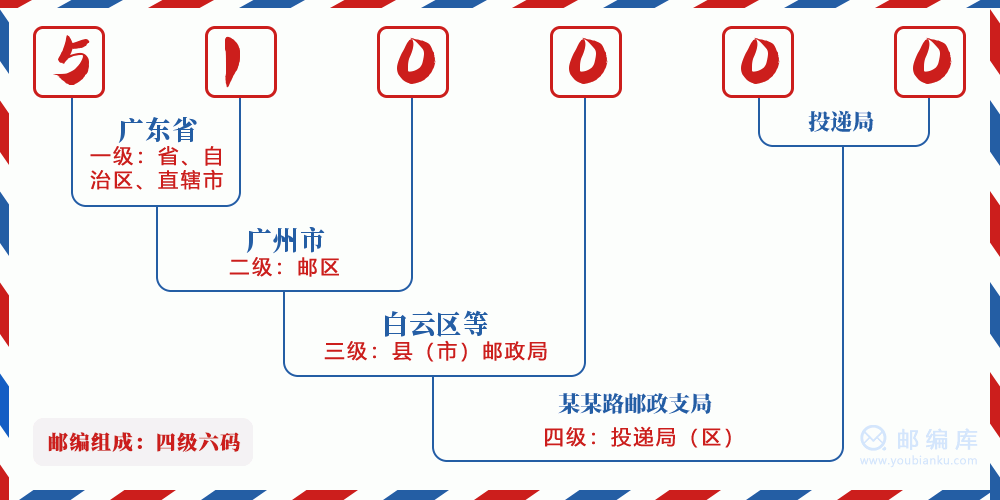
\includegraphics[width=0.9\linewidth]{./figures/FIG0.PNG}
      \end{figure}
    \end{minipage}
    \hfill
    \begin{minipage}[c]{0.6\linewidth}
      \begin{figure}
        \centering
        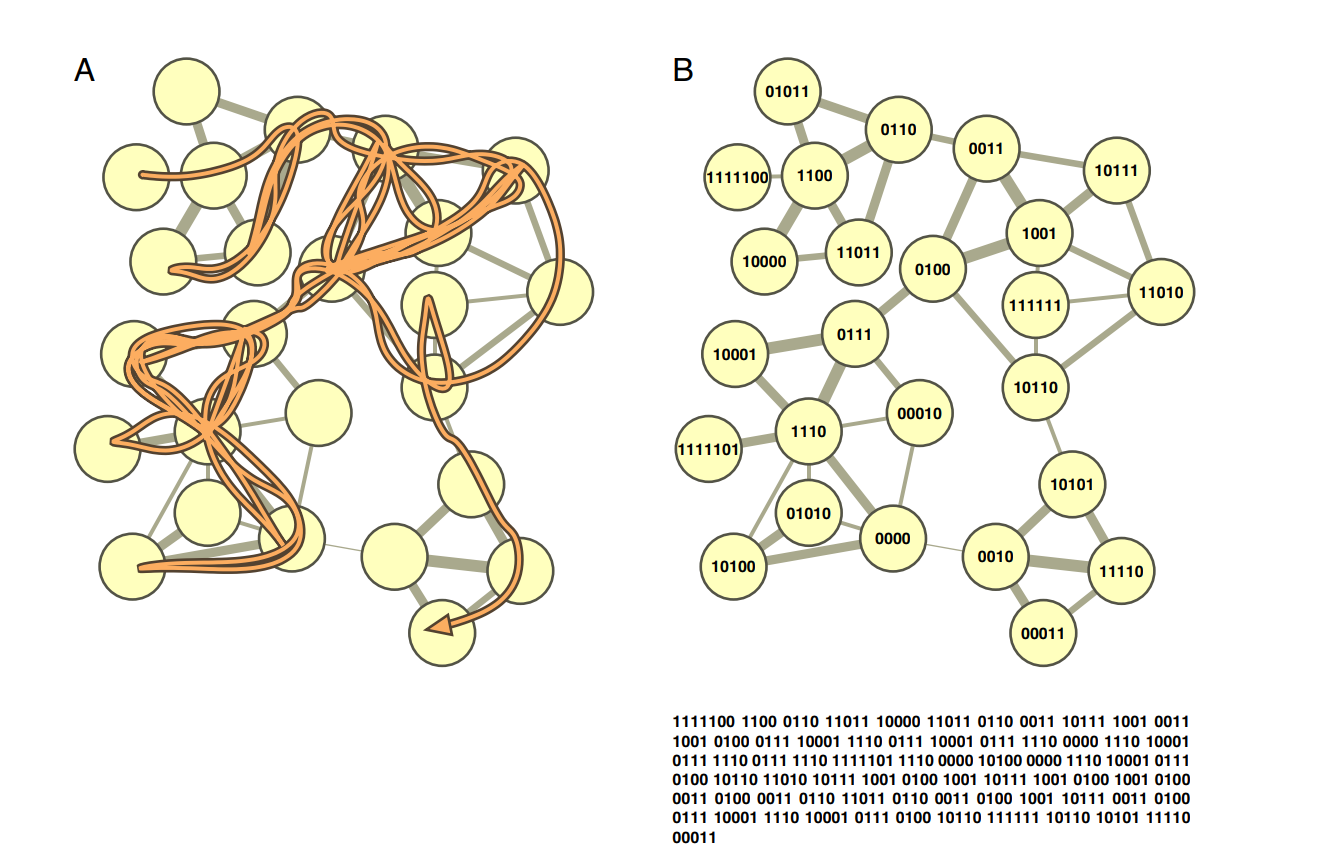
\includegraphics[width=0.9\linewidth]{./figures/FIG1.PNG}
      \end{figure}
    \end{minipage}
  \end{frame}

  \begin{frame}{Random Walk and Coding Theory}
    \begin{figure}
      \centering
      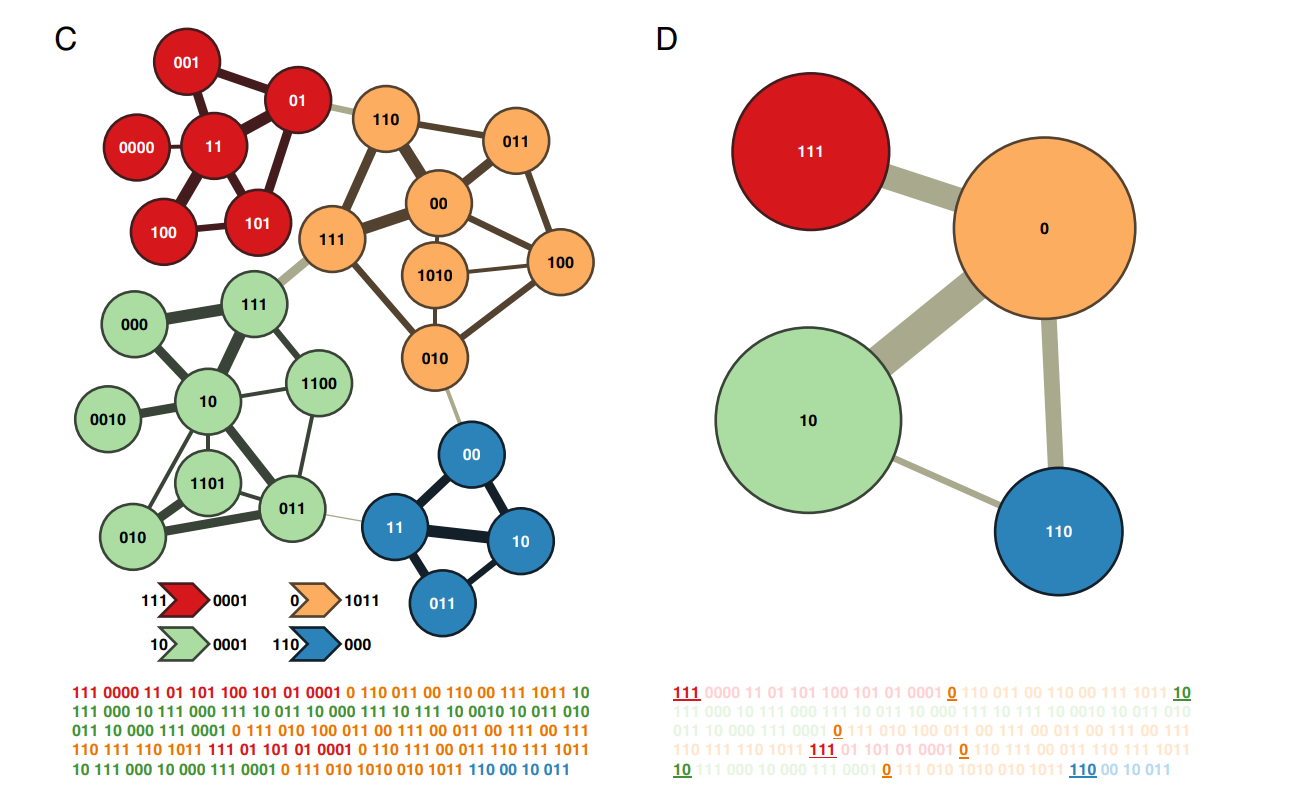
\includegraphics[width=0.7\textwidth]{./figures/FIG2.png}
    \end{figure}
  \end{frame}

\section{Existing Measures of Graph Entropy}
  \begin{frame}{Global Measures}
    For a connected graph $G$ with $n$ nodes,
    \begin{equation}
      \mathcal{I}(G) = -\sum_{i=1}^{k} \frac{n_i}{n} \log_{2} \frac{n_i}{n}.
    \end{equation}
    where $n_i$ is the number of topologically equivalent vertices in the $i$-th vertex orbits of $G$, 
    and $k$ is the number of different orbits.
  \end{frame}

  \begin{frame}{Local Entropy Measures}
    For each $i$, define the entropy of $i$ in $G$ by
    \begin{equation}
      \mathcal{I}^{G}(i) = -\sum_{j=1}^{n} \frac{d(i,j)}{d(i)} \log_2 \frac{d(i,j)}{d(i)}.
    \end{equation}
    where $d(i,j)$ is the distance between $i$ and $j$ in $G$, and $d(i)$ is the sum of $d(i,j)$ for all $j$.
  \end{frame}

  \begin{frame}{Parametric Graph Entropy}
    Given a network $G=(V,E)$ and a function $f$ from $V$ to positive real numbers, define
    \begin{equation}
      p(i) = \frac{f(i)}{\sum_{j=1}^{n}f(i)}.
    \end{equation}
    \vspace{0.2cm}
    \alert{The parametric measure is the Shannon entropy of the distribution $(p(1),p(2),\cdots,p(n))$.}
  \end{frame}

  \begin{frame}{Gibbs Entropy}
    Given a microcanonical ensemble, the Gibbs entropy is defined as
    \begin{equation}
      \Sigma = \frac{1}{n} \log N.
    \end{equation}
    where $N$ is the number of the networks in the ensemble. \\
    \vspace{0.2cm}
    \alert{The Gibbs entropy of a network ensemble is the number of bits needed to determine the code 
    of the network generated by the ensemble.} \\
    \vspace{0.2cm}
    $\diamond$ ensemble \\
    $\diamond$ microcanonical ensemble \\ 
  \end{frame}

  \begin{frame}{Shannon Entropy}
    For a network of $n$ nodes, in which each pair of nodes $(i,j)$ of weight $\alpha$ is created with probability 
    $\pi_{ij}(\alpha)$. Then the probability of the canonical undirected network ensemble, which is defined by its 
    adjacency matrix ${a_{i,j}}$, is defined by
    \begin{equation}
      \mathbf{\Pi} = \prod_{i < j} \pi_{i,j} (a_{i,j}),  \notag
    \end{equation}
    for which the log-likelihood function is given by
    \begin{equation}
      \mathcal{L} = - \sum_{i < j} \log \pi_{i,j}(a_{i,j}).  \notag
    \end{equation}
  \end{frame}

  \begin{frame}{Shannon Entropy}
    The entropy of a canonical ensemble is defined as
    \begin{equation}
      S = \langle \mathcal{L} \rangle_{\mathbf{\Pi}} = - \sum_{i < j} \sum_{\alpha} \pi_{i,j}(\alpha) \log \pi_{i,j}(\alpha).
    \end{equation}
    For undirected network where $\alpha=0,1$,
    \begin{equation}
      S = - \sum_{i < j} p_{i,j} \log p_{i,j} - \sum_{i < j} (1-p_{i,j}) \log (1-p_{i,j}),  \notag
    \end{equation}
    where $p_{i,j}=\pi_{i,j}(1)$ is the probability of the existence of the edge $(i,j)$. \\
    \vspace{0.2cm}
    \alert{The Shannon entropy of a network ensemble is the number of bits needed to determine the expression of 
    the network generated by the ensemble.}
  \end{frame}

  \begin{frame}{Von Neumann Entropy}
    Define a dense matrix as
    \begin{equation}
      \rho = L / \sum_{i,j} a_{i,j},  \notag
    \end{equation}
    where $L$ is the Laplacian matrix of the network with $L_{i,j} = \sum_{r} a_{ir} \delta_{i,j} - a_{a,j}$. \\
    \vspace{0.2cm}
    Define the von Neumman entropy of an ensemble as
    \begin{equation}
      S_{VN} = - \langle {\rm Tr} \rho \log \rho \rangle_{\mathbf{\Pi}}.
    \end{equation}
  \end{frame}

  \begin{frame}{Structural Entropy of Models of Networks}
    Given a random graph model $\mathcal{M}$, let $\mathcal{S}$ be the set of all graphs of the same type~(isomorphic)
    generated by model $\mathcal{M}$. 
    The structural entropy $H_{\mathcal{S}}$ of $\mathcal{S}$ is the Shannon entropy of the distribution $p(G)$ for all 
    $G \in \mathcal{S}$, 
    \begin{equation}
      H_{\mathcal{S}} = - \sum_{G \in \mathcal{S}} p(G) \log p(G),
    \end{equation}
    where $p(G)$ is the probability of generating a graph $G$ by the model $\mathcal{M}$. \\
  \end{frame}


\section{The Challenges}
  \begin{frame}{Quantification of Structural Information}
    \begin{minipage}[c]{0.45\linewidth}
      \begin{figure}
        \centering
        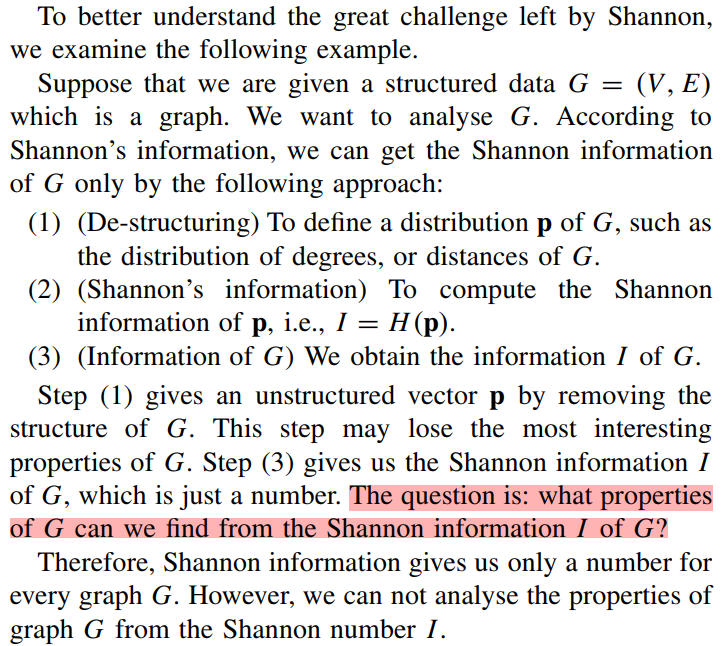
\includegraphics[width=0.9\linewidth]{./figures/FIG3.PNG}
      \end{figure}
    \end{minipage}
    \hfill
    \begin{minipage}[c]{0.45\linewidth}
      \begin{figure}
        \centering
        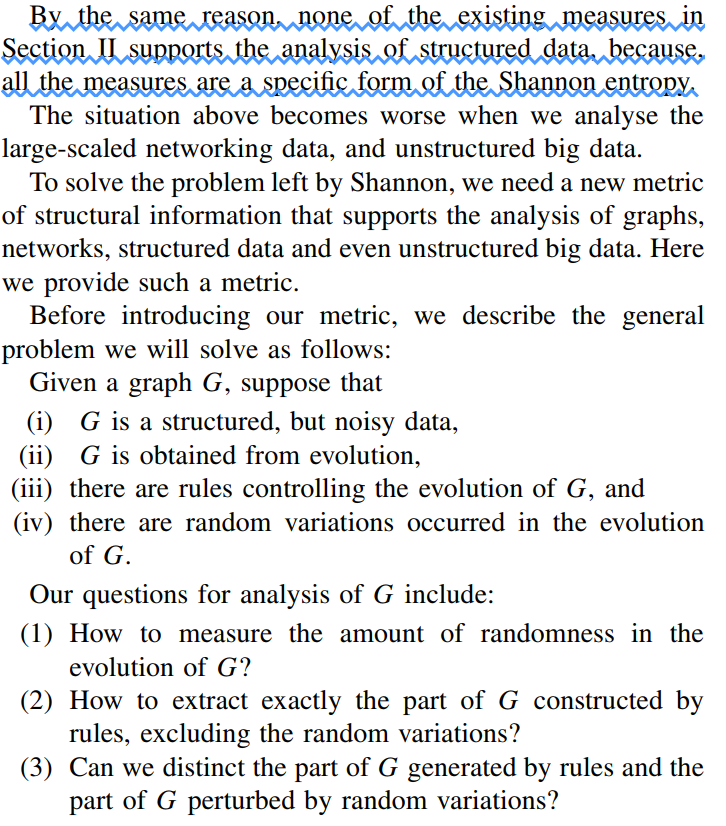
\includegraphics[width=0.8\linewidth]{./figures/FIG4.PNG}
      \end{figure}
    \end{minipage}
  \end{frame}

  \begin{frame}{Dynamical Complexity of Networks}
    \begin{enumerate}
      \item Networks are complex. How to measure this complexity?
      \item Naturally evolving networks are hard even to describe, to define or to store. All the existing notions of various entropy can be regarded as static measures of complexity.
      \item The great challenge: measure the complexity of interactions, communications, operations and evolution of the real world networks.
      \item Evolving in two ways: nature/society v.s. engineered.
    \end{enumerate}
    \vspace{0.3cm}
    \textbf{Question:} What is the dynamical complexity of networks?
  \end{frame}

\section{Overall Ideas}
  \begin{frame}{Intuition}
    Given a noisy or corrupted graph $G$, define the structural information $H$, the essential structure $T$, the true knowledge $K$.
    \begin{enumerate}
      \item $K$ is placed in $T$.
      \item $T$ is determined by $H$.
      \item $K$ consists of the rules, regulations and laws of $G$.
      \item $T$ is obtained from $G$ by excluding the maximum amount of nondeterminism, uncertainty, and noise that occurred in $G$.
    \end{enumerate}
  \end{frame}

  \begin{frame}{Inspiration}
    \begin{minipage}[c]{0.45\linewidth}
      \begin{figure}
        \centering
        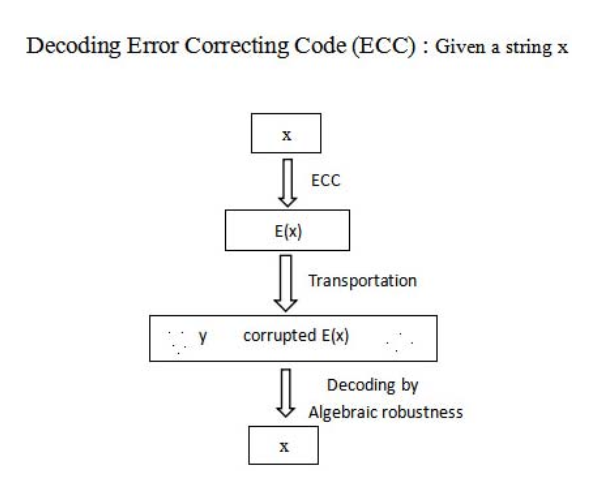
\includegraphics[width=0.9\linewidth]{./figures/FIG5.PNG}
      \end{figure}
    \end{minipage}
    \hfill
    \begin{minipage}[c]{0.45\linewidth}
      \begin{figure}
        \centering
        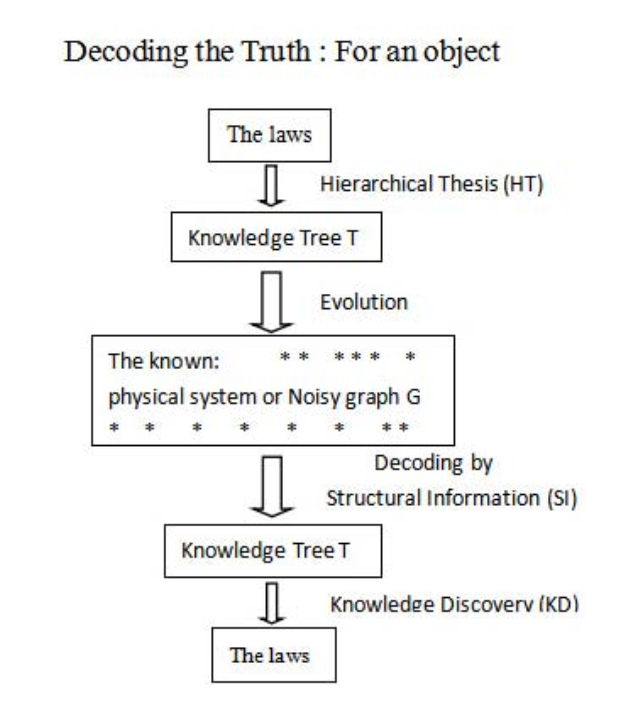
\includegraphics[width=0.8\linewidth]{./figures/FIG6.PNG}
      \end{figure}
    \end{minipage}
  \end{frame}

  \begin{frame}{Steps:}
    Given an object, suppose
    \begin{enumerate}
      \item Unknown laws of the object.
      \item Hierarchical Thesis.
      \item Physical or noisy graph.
      \item Decoding by structural information.
      \item Knowledge discovery.
    \end{enumerate}
  \end{frame}


\section{Graph Structural Information}
  \begin{frame}{One-Dimensional Structural Information}
    \begin{exampleblock}{Definition 1~(One-Dimensional Structural Information of Connected and Undirected Graphs)}
      Let $G=(V, E)$ be an undirected and connected graph with $n$ nodes and $m$ edges.
      For each node $i \in (1,2,\cdots,n)$, let $d_i$ be the degree of node $i$ in $G$, and let $p_i=\frac{d_i}{2m}$. \\
      Then the stationary distribution of the random walk in $G$ is described by probability verctor $\bm{p}=(p_1,p_2,\cdots,p_n)$.
      Define the one-demisional structural information of $G$ or the positioning entropy of $G$ as follows:
      \begin{equation}
        \begin{aligned}
          \mathcal{H}^{1}(G) &= H(\bm{p}) = H\left( \frac{d_1}{2m},\cdots,\frac{d_2}{2m} \right) \\
                             &= - \sum_{i=1}^{n} \frac{d_i}{2m} \log_{2} \frac{d_i}{2m}
        \end{aligned}
      \end{equation} 
    \end{exampleblock}
    It measures the information required to determine the one-demisional code of the node that is accessible from random walk in $G$ with stationary distribution.
  \end{frame}

  \begin{frame}{One-Dimensional Structural Information}
    \begin{exampleblock}{Definition 2~(Weighted Degree and Volume)}
      Given a network $G=(V, E)$, suppose that the weights assigned to edges is defined by a weight function $w: E \rightarrow \mathbb{R}^{+}$.
      Define the weighted degree of node $u$ to be 
      \begin{equation}
        d_{u}=\sum_{v \in N(u)} w((u,v)), \notag
      \end{equation}
      where $N(u)$ is the set of neighbors of $u$. 
      A weighted graph has $k$-bounded weight if for every edge $e$, $w(e) \leq k$.
      For a subset $U \subseteq V$, define the volume of $U$ to be
      \begin{equation}
        vol(U) = \sum_{v \in U} d_{v}. \notag
      \end{equation}
      Define the volume of $G$ to be $vol(G) = \sum_{v \in V} d_{v}$.
    \end{exampleblock}
  \end{frame}

  \begin{frame}{One-Dimensional Structural Information}
    \begin{exampleblock}{Definition 3~(One-Dimensional Structural Information of Weighted and Connected Networks)}
      Let
    \end{exampleblock}
  \end{frame}

  \begin{frame}{One-Dimensional Structural Information}
    \begin{exampleblock}{Definition 4~(One-Dimensional Structural Information of Directed and Connected Graph)}
      Given
    \end{exampleblock}
  \end{frame}
  
  \begin{frame}{One-Dimensional Structural Information}
    \begin{exampleblock}{Definition 5~(One-Dimensional Structural Information of Disconnected Graphs)}
      Given
    \end{exampleblock}
  \end{frame}

\section*{Thank you}
  \begin{frame}{}
    \begin{figure}
      
\includegraphics[width=1.0\textwidth]{./figures/thank_you.png}
    \end{figure}
  \end{frame}

\end{document}
